\documentclass{beamer} % Использование класса beamer для создания презентации
\usetheme{Boadilla} % Применение темы Boadilla

\usepackage[T2A]{fontenc} % Установка кодировки шрифта
\usepackage[utf8]{inputenc} % Установка кодировки исходного текста
\usepackage[english,russian]{babel} % Подключение локализации и переносов для русского и английского языков
\usepackage{amsmath,amssymb} % Подключение математических символов и формул
\usepackage{autonum} % Автоматическая нумерация формул только при наличии ссылок на них
\usepackage{wrapfig} % Подключение пакета для обтекания текстом рисунков и таблиц
\usepackage{array} % Подключение пакета для работы с таблицами

\newcommand{\PreserveBackslash}[1]{\let\temp=\\#1\let\\=\temp} % Команда для сохранения обратной косой черты в ячейках таблицы
\newcolumntype{C}[1]{>{\PreserveBackslash\centering}p{#1}} % Создание нового типа столбца с центрированным содержимым

\usepackage[labelformat=empty]{caption} % Подключение пакета для настройки подписей и удаление названия "Рисунок"
\graphicspath{{./images/}} % Указание папок, где искать изображения

\setbeamertemplate{navigation symbols}{} % Удаление навигационных символов на слайдах
\usepackage{ragged2e} % Подключение пакета для улучшенного выравнивания текста
\newcommand{\jj}{\righthyphenmin=20 \justifying} % Команда для активации выравнивания по ширине с установкой минимального количества символов в слове перед переносом

\date{\today}

\begin{document}

\begin{frame}
  \begin{center}\tiny
    Федеральное государственное автономное образовательное учреждение высшего образования \\
    «Национальный исследовательский университет ИТМО»\\
    Факультет систем управления и робототехники
  \end{center}

  \begin{center}\tiny
    \textbf{\MakeUppercase{ВЫПУСКНАЯ КВАЛИФИКАЦИОННАЯ РАБОТА БАКАЛАВРА \\ ПО НАПРАВЛЕНИЮ 15.03.06 <<Мехатроника и робототехника>>}}\\
    \vspace{0.2cm}
    \textbf{\MakeUppercase{на тему:}}\\
    \vspace{0.1cm}
    \textbf{\MakeUppercase{<<Исследование и сравнение современных алгоритмов
    компьютерного зрения \\ для отслеживания перемещения объектов на видеоизображениях в
    городской среде>>}}
  \end{center}

  \vspace{0.3cm}

  \begin{columns}
    \begin{column}{0.50\textwidth}
      \begin{center}\tiny
        Выполнил: \\
        \vspace{0.1cm}
        \textbf{Лалаянц Кирилл Артемович}\\
        студент группы R34352 \\
        336700\\
      \end{center}
    \end{column}

    \begin{column}{0.50\textwidth}
      \begin{center}\tiny
        Научный руководитель:\\
        \vspace{0.1cm}
        \textbf{Шаветов Сергей Васильевич} \\
        доцент, к.т.н., заместитель декана ФСУиР\\
        начальник ДНИР \\
      \end{center}
    \end{column}
  \end{columns}

  \vspace{0.5cm}
  \begin{center}\tiny
    Санкт-Петербург \\
    $2025$
  \end{center}
\end{frame}

\begin{frame}{Цель работы и практическая значимость}
  \begin{itemize}
    \item \textbf{Цель:} Исследовать возможность запуска методов отслеживания объектов на видеоизображениях на малопроизводительных устройствах с сохранением высокого качества и высокой скоростью обработки.
    \item \textbf{Практическая значимость:}
      \begin{itemize}
        \item Разработка рекомендаций по выбору алгоритмов для реального времени.
        \item Повышение эффективности систем автономного управления и анализа данных.
      \end{itemize}
  \end{itemize}
  % Дополнительно можно добавить схематическое изображение или пиктограмму, отражающую реальное время и автономность.
  % \vspace{0.3cm}
  % \centering
  % \includegraphics[width=0.3\linewidth]{review/low_power_device.png}
\end{frame}


\begin{frame}{Постановка задачи отслеживания}
  \begin{itemize}
    \item Обработка видеоизображений для извлечения информации об объектах:
      \begin{itemize}
        \item Детектирование объектов
        \item Присвоение уникальных идентификаторов
        \item Сохранение истории перемещений
      \end{itemize}
    \item Ключевые подходы:
      \begin{itemize}
        \item MOT (Multiple Object Tracking) и SOT (Single Object Tracking)
        \item Online и offline методы
        \item Двухкомпонентные системы – оптимальный выбор для маломощных устройств
      \end{itemize}
  \end{itemize}
  % Если имеется диаграмма, иллюстрирующая эти этапы, можно добавить её ниже:
  % \vspace{0.5cm}
  % \centering
  % \includegraphics[width=0.5\linewidth]{path_to_tracking_pipeline_diagram.png}
\end{frame}

\begin{frame}{Актуальность}
  \begin{columns}[T]
    \begin{column}{\textwidth}
      \textbf{Спортивная аналитика:}
      \begin{itemize}
        \item Отслеживание траекторий мяча
      \end{itemize}
    \end{column}
    % \begin{column}{0.5\textwidth}
    %   \textbf{Зоология:}
    %   \begin{itemize}
    %     \item Анализ поведения животных
    %   \end{itemize}
    % \end{column}
  \end{columns}
  \vspace{0.5cm}
  \begin{columns}
    \begin{column}{0.5\textwidth}
      \centering
      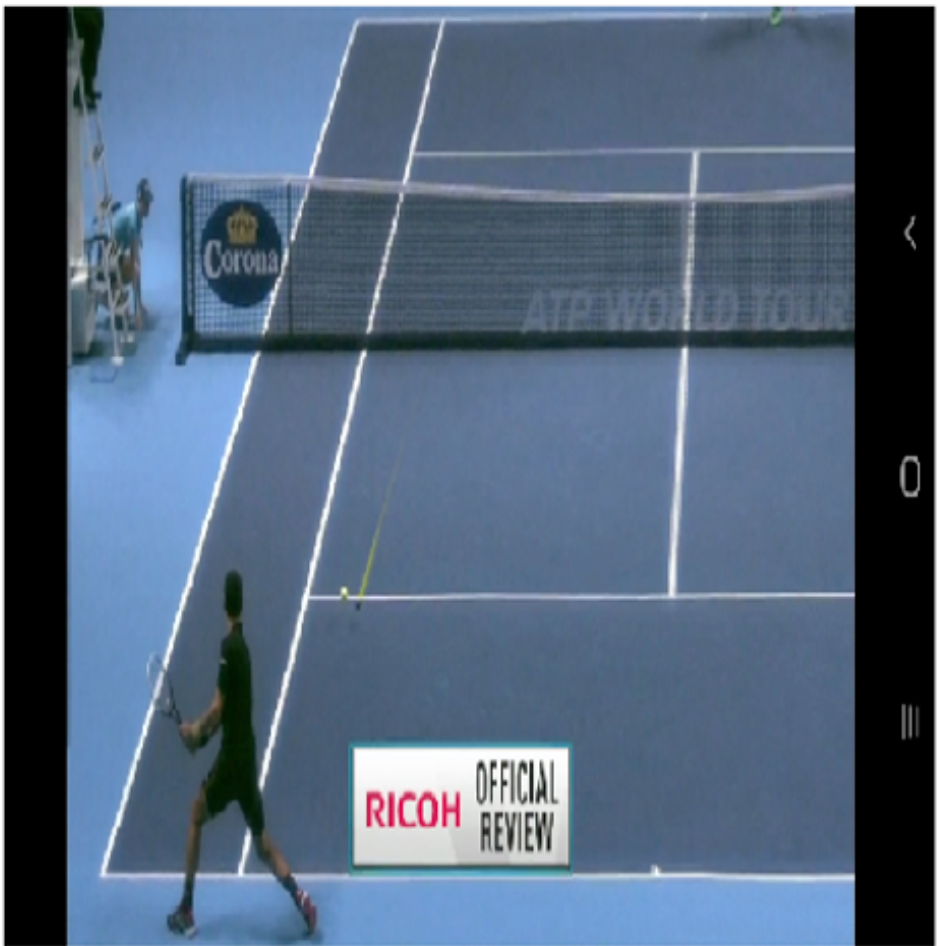
\includegraphics[width=\linewidth]{review/ball_track.png}
      \small Спортивная аналитика
    \end{column}
    % \begin{column}{0.5\textwidth}
    %   \centering
    %   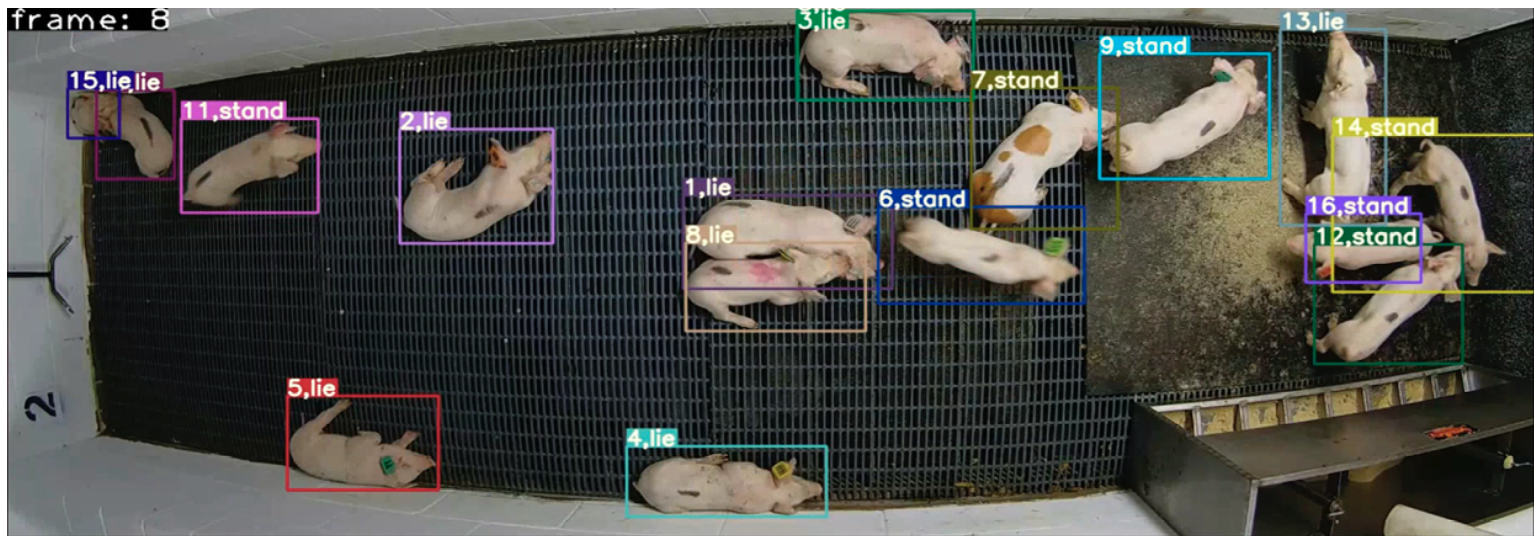
\includegraphics[width=\linewidth]{review/animals.png}
    %   \small Зоология
    % \end{column}
  \end{columns}
\end{frame}

\begin{frame}{Актуальность}
  \textbf{Урбанистика:}
  \begin{itemize}
    \item Подсчёт автомобилей и анализ движения на городских улицах
  \end{itemize}
  \vspace{0.5cm}
  \centering
  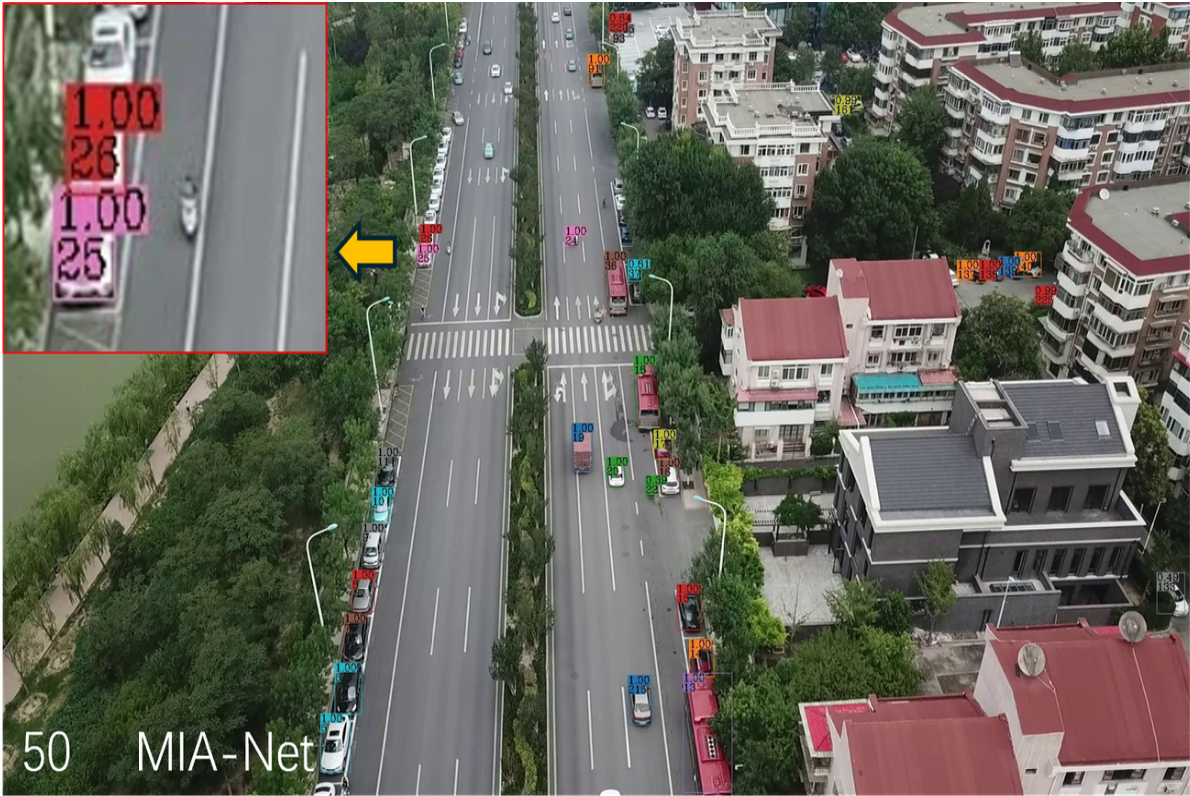
\includegraphics[width=0.7\linewidth]{review/urban_uav.png}\\
  \small Урбанистический анализ с использованием БПЛА
\end{frame}

\begin{frame}{Актуальность}
  \textbf{Робототехника:}
  \begin{itemize}
    \item Обеспечение навигации и безопасности
    \item Следование за объектом
  \end{itemize}
  \vspace{0.5cm}
  \centering
  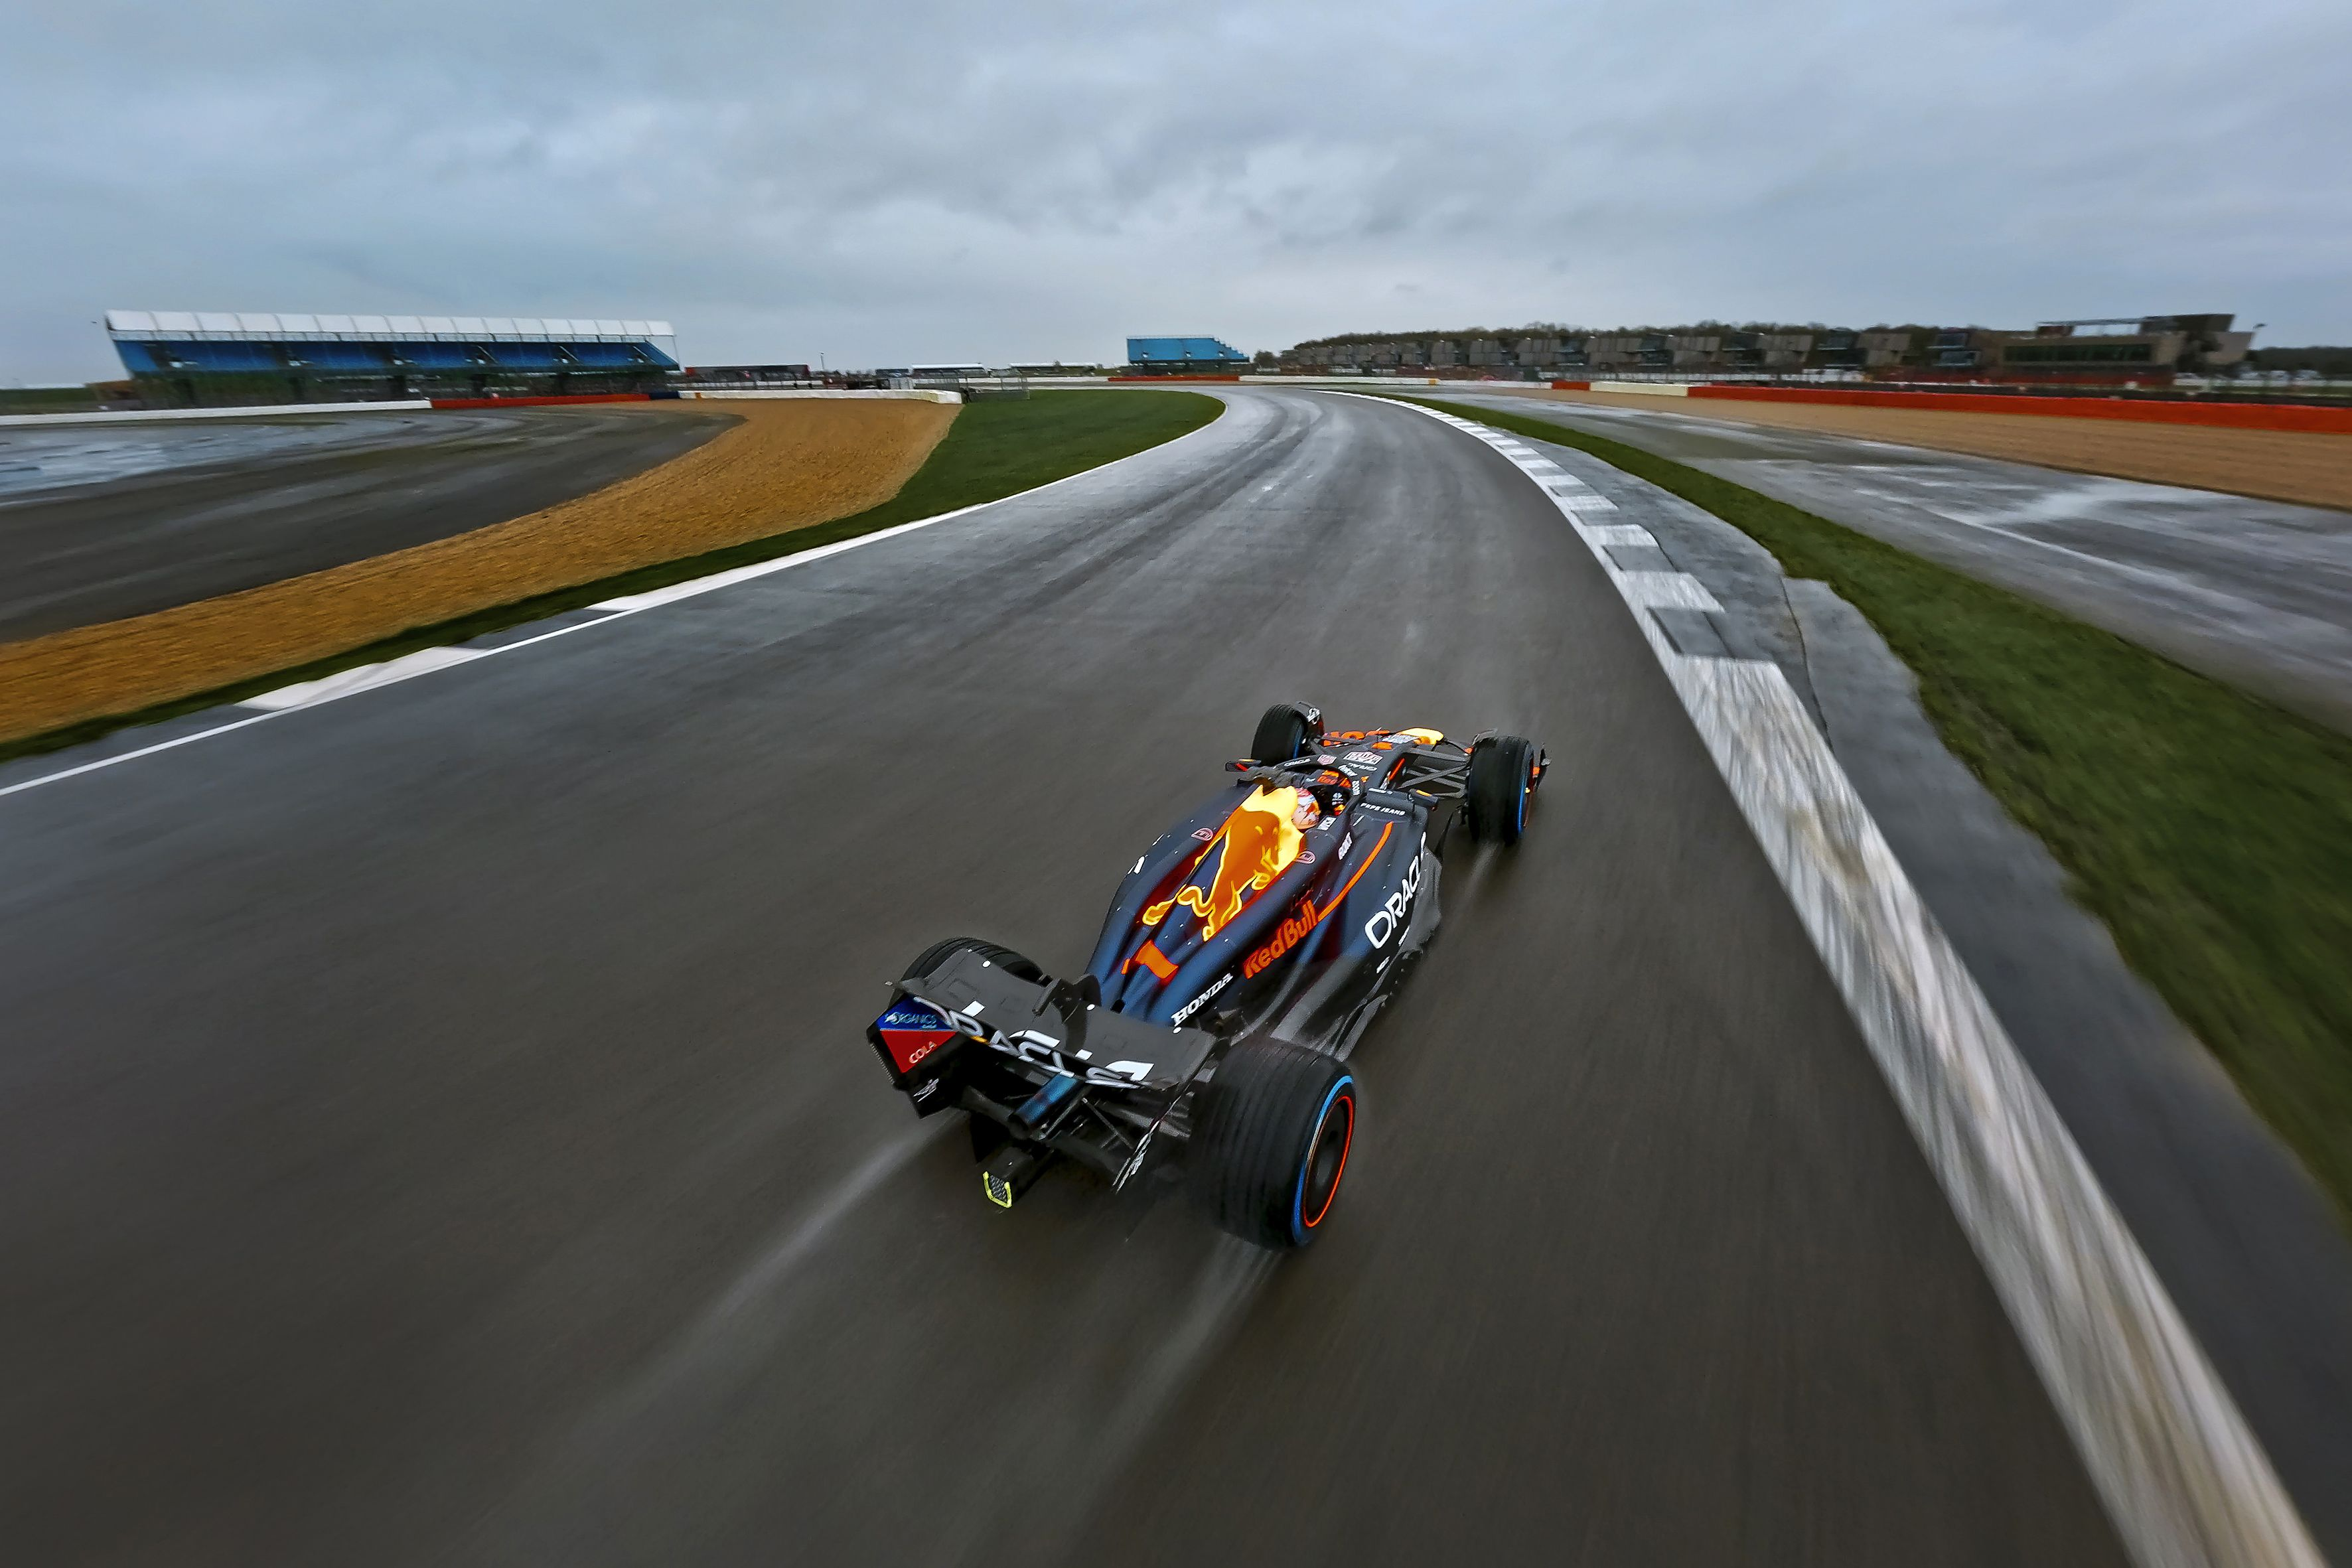
\includegraphics[width=0.7\linewidth]{presentation/f1_car.jpg}\\
  \small Кадр дрона оператора гонки F1
\end{frame}

\begin{frame}{Цель работы и практическая значимость}
  \begin{columns}[T]
    \begin{column}{0.45\textwidth}
      \textbf{Проблемы:}
      \begin{itemize}
        \item Высокие требования к вычислительным ресурсам
        \item Задержки при централизованной обработки
        \item Риски потери данных и сбоев соединения
      \end{itemize}
    \end{column}
    \begin{column}{0.45\textwidth}
      \textbf{Решение:}
      \begin{itemize}
        \item Использование микрокомпьютера
        \item Локальная обработка данных в реальном времени
        \item Повышение автономности и отказоустойчивости системы
      \end{itemize}
    \end{column}
  \end{columns}
\end{frame}



\begin{frame}{Актуальность}
  \footnotesize{

    \textbf{Актуальность:}

    Остаются открытыми такие важные вопросы, как влияние потенциала взаимодействия между частицами на температурную зависимость коэффициента диффузии и насколько важны корреляции между спектрами возбуждения частиц и транспортными свойствами, а также, какую роль играет дальнодействие притяжения в скорости нуклеации в переохлажденных системах

    \vspace{1cm}

    \textbf{Практическая значимость:}

    \begin{itemize}
    \item Чc
    \end{itemize}
  }
\end{frame}




\begin{frame}{Цель и задачи работы}
  \footnotesize{

    \textbf{Цель работы} -- 

    \vspace{0.5cm}

    \textbf{Задачами работы являются:}
    \begin{itemize}
    \item Расчет
    \end{itemize}
  }
\end{frame}


\begin{frame}
  \centering \Huge \textcolor{blue}{Спасибо за внимание!}
\end{frame}

\end{document}
